
In TSF only the original/time-domain representation of a time series is looked at.
To capture a broader range of discriminations STSF uses multiple representations.
\subsubsection*{Periodogram}
Using a discrete Fourier transform the time series is mapped into the 
frequency domain. This allows STSF to detect intervals with discriminative periodic patterns,
even if they occur at varying time points across instances. "A side benefit of this 
representation is that it helps to indirectly detect phase-independent discriminatory intervals, i.e.m
discriminatory features located at different time regions of the original series as described in 
\Cref{fig:perio}" 

\begin{figure}[h]
\centering
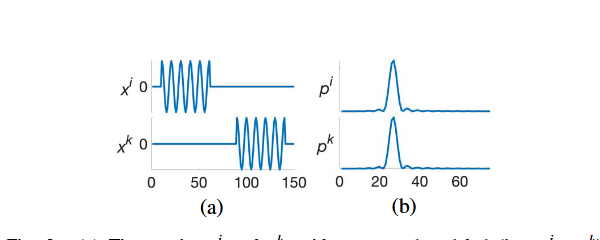
\includegraphics[width=\linewidth]{res/periobullshit.png}
\caption{"(a) Time series $x^i$ and $x^k$, with a same class label (i.e., $y^i = y^k$)
present a similar sub-series but located at different time regions (i.e., phase-
independent). (b) The periodogram representation $p^i$ and $p^k$ of series $x^i$ and
$x^k$, respectively. Our algorithm searches for discriminatory phase-dependent
interval features and cannot find discriminatory intervals that identify both
series as similar. The periodogram representation provides more flexibility
as it considers the frequency of the discriminatory sub-series (ignoring its
location in time) and thus helps to identify discriminatory sub-series even
when they appear at different locations in time across different time series."} % TODO: ref
\label{fig:perio}
\end{figure}
\subsubsection*{Derivative representation}
STSF also adopts the derivative representation as one of three complementary views 
on the input time series. The derivative captures local trends. This view emphasizes hte shape or dynamic behavior of the 
series over absolute levels. "The
discrete derivative of a time series $f$ with length $n$ is defined by
\[
	f'(i) = f(i) - f(i - 1) \forall ~ i \in \{2,3, \dots, n\}
\] %TODO: cite derivative

